\documentclass[answers]{exam}

\usepackage[utf8]{inputenc}
\usepackage{amsmath, amssymb}
\usepackage{bm}
\usepackage{color}
\usepackage{caption}
\usepackage{enumitem}
\usepackage{float}
\usepackage{graphicx}
\usepackage{listings}
\usepackage{mathtools}
\usepackage{tikz}

\definecolor{keyblue}{rgb}{0.1, 0.1, 0.6}
\definecolor{dkgreen}{rgb}{0,0.6,0}
\definecolor{gray}{rgb}{0.5,0.5,0.5}
\definecolor{stringcol}{rgb}{0.58,0.4,0.1}

\DeclareCaptionFormat{listing}
    {\colorbox[cmyk]{0.73, 0.35, 0.15,.5}
    {\parbox{\dimexpr\textwidth-2\fboxsep\relax}{#1#2#3}}}
\DeclareCaptionFont{white}{\color{white}}
\captionsetup[lstlisting]{
    format=listing,
    labelfont=white,
    textfont=white,
    font={bf,footnotesize}
}

\lstset{
    language=R,
    columns=flexible,
    basicstyle={\small\ttfamily},
    keywordstyle=\color{keyblue},
    commentstyle=\color{dkgreen},
    stringstyle=\color{stringcol},
    breaklines=true,
    breakatwhitespace=true,
    tabsize=4
}

\usetikzlibrary{shapes, arrows, positioning}

\begin{document}
\title{Proses Stokhatik: UAS}
\author{GitHub : FadhlyAzka}
\date{2024/2025}

\maketitle

\begin{lstlisting}[title=Code]
suppressWarnings(suppressMessages(library(diagram)))
suppressWarnings(suppressMessages(library(expm)))
suppressWarnings(suppressMessages(library(markovchain)))
\end{lstlisting}

\begin{questions}
    \question Consider two drunken symbols, Club ($\clubsuit$) and Spade ($\spadesuit$), walking along the streets given by the following diagram:
    \begin{center}
        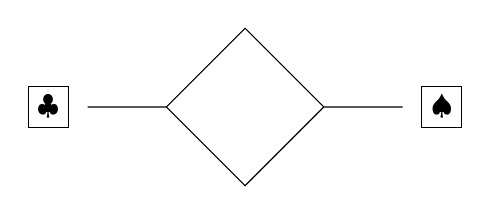
\begin{tikzpicture}{->, >=stealth', auto, line width =0.5pt}
            \node [draw] (Club) at (-0.5, 0) {$\clubsuit$};
            \node [draw] (Spade) at (4.5, 0) {$\spadesuit$};
            \draw (0,0) -- ++(1,0) -- ++(1,1) -- ++(1,-1) -- ++(1,0);
            \draw (1,0) -- ++(1,-1) -- ++(1,1);
        \end{tikzpicture}
    \end{center}
    We assume they are taking a simple random walk and are interested in determining the expected time that they will take to meet each other. After identification of equivalent positions (after rotation, mirroring, etc.), we determine that there are 6 possible states that the symbols can find themselves in that we label from 1 to 6. We assume that the two symbols start in state 1.
    
        \begin{parts}
            \part Draw the diagram transition.
                \begin{solution}

                \end{solution}
                \begin{minipage}[t]{.9\textwidth}
                    \begin{lstlisting}[title=Code]

                    \end{lstlisting}
                \end{minipage}
                \newline
                \begin{minipage}[t]{.9\textwidth}
                    \begin{lstlisting}[title=Output]

                    \end{lstlisting}
                \end{minipage}

            \part What is the expected time for them to meet?
                \begin{solution}
                    
                \end{solution}
                \begin{minipage}[t]{.9\textwidth}
                    \begin{lstlisting}[title=Code]

                    \end{lstlisting}
                \end{minipage}
                \newline
                \begin{minipage}[t]{.9\textwidth}
                    \begin{lstlisting}[title=Output]

                    \end{lstlisting}
                \end{minipage}
        \end{parts} 

    \question Consider a Markov chain with state $\textsl{S} = 0, 1, ... , 9$ with the transition probability matrix below
    $$\mathbf{P}=\left(\begin{array}{cccccccccc}0 & 0 & 0.6 & 0 & 0 & 0.4 & 0 & 0 & 0 & 0 \\ 0 & 0 & 0 & 0 & 0.7 & 0 & 0 & 0.3 & 0 & 0 \\ 0.3 & 0 & 0 & 0.5 & 0 & 0 & 0.2 & 0 & 0 & 0 \\ 0 & 0 & 0 & 0.8 & 0 & 0 & 0 & 0 & 0.2 & 0 \\ 0 & 0.4 & 0 & 0 & 0 & 0 & 0 & 0.6 & 0 & 0 \\ 0 & 0 & 0 & 0 & 0.5 & 0.2 & 0 & 0 & 0 & 0.3 \\ 0.4 & 0 & 0 & 0 & 0 & 0 & 0.3 & 0 & 0.3 & 0 \\ 0 & 0.3 & 0 & 0 & 0.7 & 0 & 0 & 0.5 & 0 & 0 \\ 0 & 0 & 0 & 0.9 & 0 & 0 & 0 & 0 & 0.1 & 0 \\ 0 & 0 & 0 & 0 & 0 & 0.5 & 0 & 0 & 0 & 0.5\end{array}\right)$$
        \begin{parts}
            \part Draw the diagram of the Markov chain. 
                \begin{solution}
                \\State space $S = \{0, 1, 2, 3, 4, 5, 6, 7, 8, 9\}$
                    \begin{center}
                        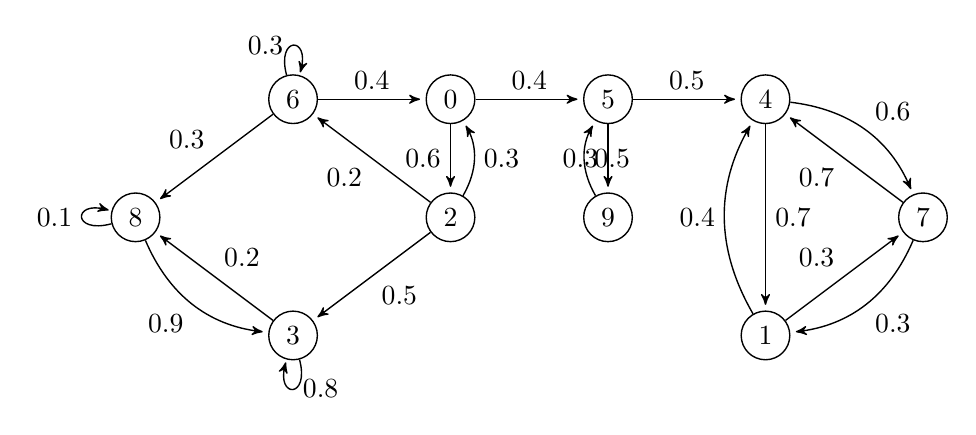
\begin{tikzpicture}[->, >=stealth', auto, semithick, shorten >=2pt, line width =0.5pt, node distance =2cm]
                            \node [circle , draw] (zero) at (-1, 1.5) {0};
                            \node [circle , draw] (one) at (3, -1.5) {1};
                            \node [circle , draw] (two) at (-1, 0) {2};
                            \node [circle , draw] (three) at (-3, -1.5) {3};
                            \node [circle , draw] (four) at (3, 1.5) {4};
                            \node [circle , draw] (five) at (1, 1.5) {5};
                            \node [circle , draw] (six) at (-3, 1.5) {6};
                            \node [circle , draw] (seven) at (5, 0) {7};
                            \node [circle , draw] (eight) at (-5, 0) {8};
                            \node [circle , draw] (nine) at (1, 0) {9};
                            \path (zero) edge node [above] {$0.4$} (five);
                            \path (two) edge node [below right] {$0.5$} (three);
                            \path (two) edge node [below left] {$0.2$} (six);
                            \path (five) edge node [above] {$0.5$} (four);
                            \path (six) edge node [above] {$0.4$} (zero);
                            \path (six) edge node [above left] {$0.3$} (eight);
                            \path (zero) edge node [left] {$0.6$} (two);
                            \path (two) edge [bend right] node [right] {$0.3$} (zero);
    
                            \path (one) edge [bend left] node [left] {$0.4$} (four);
                            \path (four) edge node [right] {$0.7$} (one);
    
                            \path (one) edge node [above left] {$0.3$} (seven);
                            \path (seven) edge [bend left] node [below right] {$0.3$} (one);
    
                            \path (three) edge node [above right] {$0.2$} (eight);
                            \path (eight) edge [bend right] node [below left] {$0.9$} (three);
    
                            \path (four) edge [bend left] node [above right] {$0.6$} (seven);
                            \path (seven) edge node [below left] {$0.7$} (four);
    
                            \path (five) edge node [left] {$0.3$} (nine);
                            \path (nine) edge [bend left] node [right] {$0.5$} (five);
    
                            \path (three) edge [loop below] node [right] {$0.8$} (three);
                            \path (six) edge [loop above] node [left] {$0.3$} (six);
                            \path (eight) edge [loop left] node [left] {$0.1$} (eight);
                        \end{tikzpicture}
                        \label{fig:markovchain_no2}
                    \end{center}

                \end{solution}
                \begin{minipage}[t]{.9\textwidth}
                    \begin{lstlisting}[title=Code]
no2.P <- matrix(c(
              0, 0, 0.6, 0, 0, 0.4, 0, 0, 0, 0,
              0, 0, 0, 0, 0.7, 0, 0, 0.3, 0, 0,
              0.3, 0, 0, 0.5, 0, 0, 0.2, 0, 0, 0,
              0, 0, 0, 0.8, 0, 0, 0, 0, 0.2, 0,
              0, 0.4, 0, 0, 0, 0, 0, 0.6, 0, 0,
              0, 0, 0, 0, 0.5, 0.2, 0, 0, 0, 0.3,
              0.4, 0, 0, 0, 0, 0, 0.3, 0, 0.3, 0,
              0, 0.3, 0, 0, 0.7, 0, 0, 0, 0, 0,
              0, 0, 0, 0.9, 0, 0, 0, 0, 0.1, 0,
              0, 0, 0, 0, 0, 0.5, 0, 0, 0, 0.5),
      nrow = 10, ncol = 10, byrow = TRUE)
no2.P

plotmat(t(no2.P),
        name = c(0, 1, 2, 3, 4, 5, 6, 7, 8, 9), shadow.size = 0, curve = 0.05,
        arr.length=0.5, arr.width=0.2, box.col="cornsilk", box.lwd=1, 
        box.prop=0.5, box.size=0.035, box.type="rect", box.cex=1, 
        cex.txt=0.7, lwd=0.5, self.cex=0.6)
                    \end{lstlisting}
                \end{minipage}
                \newline
                \begin{minipage}[t]{.9\textwidth}
                    \begin{lstlisting}[title=Output]

                    \end{lstlisting}
                \end{minipage}

            \part Find all of the communitating classes.
                \begin{solution}
                \\State i dan state j dikatakan berkomunikasi, ditulis sebagai $i \leftrightarrow j$, jika keduanya dapat diakses satu sama lain. Dalam matematika, notasi $\leftrightarrow$ diartikan sebagai \textit{equivalence relation}. Markov chain memiliki 4 kelas berkomunikasi yaitu \{0, 2, 6\}; \{1, 4, 7\}; \{3, 8\} dan \{5, 9\}
                \end{solution}
                \begin{minipage}[t]{.9\textwidth}
                    \begin{lstlisting}[title=Code]
no2.mcs <- new("markovchain", transitionMatrix = no2.P, state = as.character(0:9))
communicatingClasses(no2.mcs)
                    \end{lstlisting}
                \end{minipage}
                \newline
                \begin{minipage}[t]{.9\textwidth}
                    \begin{lstlisting}[title=Output]
[[1]]
[1] "0" "2" "6"

[[2]]
[1] "1" "4" "7"

[[3]]
[1] "3" "8"

[[4]]
[1] "5" "9"
                    \end{lstlisting}
                \end{minipage}

            \part Giving reasons, classify each state as either transient or recurrent.
                \begin{solution}
                \\Recurrent : 2 kelas = \{1, 4, 7\} dan \{3, 8\}
                \\Transient : 2 kelas = \{0, 2, 6\} dan \{5, 9\}
                \\Set dari Recurrent state $S_R = {1, 3, 4, 7, 8}$ dan set dari Transient state $S_T = {0, 2, 5, 6, 9}$
                    \begin{itemize}
                        \item Proses Markov Chain dari state Recurrent \{1, 3, 4, 7, 8\} akan selalu berputar di sekitar kelas dan tidak akan pernah keluar dari kelas tersebut
                        \item Proses Markov Chain dari state Transient \{0, 2, 5, 6, 9\} akan ada probabilitas positif dimana proses akan meninggalkan kelas dan tidak akan kembali ke kelas tersebut
                    \end{itemize}
                \end{solution}
                \begin{minipage}[t]{.9\textwidth}
                    \begin{lstlisting}[title=Code]
recurrentClasses(no2.mcs)
transientClasses(no2.mcs)
recurrentStates(no2.mcs)
transientStates(no2.mcs)                        
                    \end{lstlisting}
                \end{minipage}
                \newline
                \begin{minipage}[t]{.9\textwidth}
                    \begin{lstlisting}[title=Output]
[[1]]
[1] "1" "4" "7"

[[2]]
[1] "3" "8"

[[1]]
[1] "0" "2" "6"

[[2]]
[1] "5" "9"

[1] "1" "3" "4" "7" "8"
[1] "0" "2" "5" "6" "9"                        
                    \end{lstlisting}
                \end{minipage}
                
            \part Find the hitting probabilities to state 1 from all other states.
                \begin{solution}
                \begin{align*}
                    h_{iA} &= P(X_n \in A|X_0 = i) \\ &= 
                    \begin{cases} \sum_{j\in S} P_{ij}h_{iA} & \text{if } i\notin A \\ 1 & \text{if } i \in A
                    \end{cases}
                \end{align*}
                Dalam hal ini, A didefinisikan sebagai 1. Untuk state 1, dinyatakan $h_1 = 1$. Model menjadi:
                \begin{align*}
                    h_0 &= 0.6h_2 + 0.4h_5 \\ h_2 &= 0.3h_0 + 0.5h_3 + 0.2h_6 \\ h_3 &= 0.8h_3 + 0.2h_8 \\ h_4 &= 0.4 + 0.6h_7 \\ h_5 &= 0.5h_4 + 0.2h_5 + 0.3h_9 \\ h_6 &= 0.4h_0 + 0.3h_6 + 0.3h_8 \\ h_7 &= 0.3 + 0.7h_4 \\ h_8 &= 0.9h_3 + 0.1h_8 \\ h_9 &= 0.5h_5 + 0.5h_9
                \end{align*}
                Lakukan kalkulasi dengan software R untuk mempermudah mendapatkan output.
                \begin{align*} 
                h &= \left(\begin{array}{cccccccccc} h_0 & h_1 & h_2 & h_3 & h_4 & h_5 & h_6 & h_7 & h_8 & h_9 \end{array}\right) \\ &= \left(\begin{array}{cccccccccc} 0.5323 & 1 & 0.2205 & 0 & 1 & 1 & 0.3042 & 1 & 0 & 1 \end{array}\right)
                \end{align*}
                State {3, 8} tidak mungkin kembali ke state 1, kemudian $h_{31} = h_{81} = 0$. Model akhir berubah menjadi:
                \begin{align*}
                    h_0 &= 0.6h_2 + 0.4h_5 \\ h_2 &= 0.3h_0 + 0.2h_6 \\  h_4 &= 0.4 + 0.6h_7 \\ h_5 &= 0.5h_4 + 0.2h_5 + 0.3h_9 \\ h_6 &= 0.4h_0 + 0.3h_6  \\ h_7 &= 0.3 + 0.7h_4 \\ h_9 &= 0.5h_5 + 0.5h_9
                \end{align*}
                dengan penyelesaian, $h_{01} = 0.5353, h_{21} = 0.2205, h_{61} = 0.3042, h_{41} = h_{51} = h_{71} = h_{91} = 1$
                \end{solution}
                \begin{minipage}[t]{.9\textwidth}
                    \begin{lstlisting}[title=Code]
no2.hit_prob = hittingProbabilities(no2.mcs)
round(no2.hit_prob[,2], 4)  
                    \end{lstlisting}
                \end{minipage}
                \newline
                \begin{minipage}[t]{.9\textwidth}
                    \begin{lstlisting}[title=Output]
     0      1      2      3      4      5      6      7      8      9 
0.5323 1.0000 0.2205 0.0000 1.0000 1.0000 0.3042 1.0000 0.0000 1.0000 
                    \end{lstlisting}
                \end{minipage}

                
            \part Find and discuss the long-run behaviour (i.e. long run proportion and limiting probabilities) of the chain.
                \begin{solution}
                \begin{align*} \pi_j = \sum_i \pi_i P_{ij} \end{align*}
                Dengan syarat $\sum_j \pi_j = 1$, maka berlaku $\pi_0 + \pi_1 + \pi_2 + \pi_3 + \pi_4 + \pi_5 + \pi_6 + \pi_7 + \pi_8 + \pi_9 = 1$
                \begin{align*}
                    \pi_0 &= 0.6\pi_2 + 0.4\pi_5 \\ \pi_1 &= 0.7\pi_4 + 0.3\pi_7 \\ \pi_2 &= 0.3\pi_0 + 0.5\pi_3 + 0.2\pi_6 \\ \pi_3 &= 0.8\pi_3 + 0.2\pi_8 \\ \pi_4 &= 0.4\pi_1 + 0.6\pi_7 \\ \pi_5 &= 0.5\pi_4 + 0.2\pi_5 + 0.3\pi_9 \\ \pi_6 &= 0.4\pi_0 + 0.3\pi_6 + 0.3\pi_8 \\ \pi_7 &= 0.3\pi_1 + 0.7\pi_4 \\ \pi_8 &= 0.9\pi_3 + 0.1\pi_8 \\ \pi_9 &= 0.5\pi_5 + 0.5\pi_9
                \end{align*}
                    \begin{itemize}
                        \item Jika proses Markov Chain dimulai dari kelas Recurrent \{3, 8\}, maka limiting probabilities [0 \quad0 \quad0 \quad0.8182 \quad0 \quad0 \quad0 \quad0 \quad0.1818 \quad0]
                        \item Jika proses Markov Chain dimulai dari kelas Recurrent \{1, 4, 7\}, maka limiting probabilities [0 \quad0.2624 \quad0 \quad0 \quad0.4118 \quad0 \quad0 \quad0.3258 \quad0 \quad0]
                        \item Jika proses Markov Chain dimulai dari kelas Transient \{5, 9\}, dengan $h_{5, 9} = 1$, proses hanya bisa masuk ke kelas Recurrent {1, 4, 7}
                        \item Jika proses Markov Chain dimulai dari kelas Transient \{0, 2, 6\}, proses akan mendapatkan hasil yang berbeda
                        \begin{itemize}
                            \item Hitting probabilities dari state \{0\} ke kelas Recurrent \{3, 8\} yaitu 0.4677 dan ke kelas Recurrent \{1, 4, 7\} yaitu 0.5323 dari limiting probabilities [0 \quad0.1397 \quad0 \quad0.3826 \quad0.2192 \quad0 \quad0 \quad0.1734 \quad0.085 \quad0]
                            \item Hitting probabilities dari state \{2\} ke kelas Recurrent \{3, 8\} yaitu 0.7794 dan ke kelas Recurrent \{1, 4, 7\} yaitu 0.2206 dari limiting probabilities [0 \quad0.0579 \quad0 \quad0.6377 \quad0.0908 \quad0 \quad0 \quad0.0718 \quad0.1417 \quad0]
                            \item Hitting probabilities dari state \{6\} ke kelas Recurrent \{3, 8\} yaitu 0.6958 dan ke kelas Recurrent \{1, 4, 7\} yaitu 0.3042 dari limiting probabilities [0 \quad0.0798 \quad0 \quad0.5693 \quad0.1253 \quad0 \quad0 \quad0.0991 \quad0.1265 \quad0]
                        \end{itemize}
                    \end{itemize}
                \end{solution}
                \begin{minipage}[t]{.9\textwidth}
                    \begin{lstlisting}[title=Code]
round(steadyStates(no2.mcs), 4)

Sol2.e1 = c(no2.hit_prob[1,4], no2.hit_prob[1,5]) %*% steadyStates(no2.mcs)
Sol2.e2 = c(no2.hit_prob[3,4], no2.hit_prob[3,5]) %*% steadyStates(no2.mcs)
Sol2.e3 = c(no2.hit_prob[7,4], no2.hit_prob[7,5]) %*% steadyStates(no2.mcs)
round(Sol2.e1, 4)
round(Sol2.e2, 4)
round(Sol2.e3, 4)
                    \end{lstlisting}
                \end{minipage}
                \newline
                \begin{minipage}[t]{.9\textwidth}
                    \begin{lstlisting}[title=Output]
     0      1 2      3      4 5 6      7      8 9
[1,] 0 0.0000 0 0.8182 0.0000 0 0 0.0000 0.1818 0
[2,] 0 0.2624 0 0.0000 0.4118 0 0 0.3258 0.0000 0
     0      1 2      3      4 5 6      7     8 9
[1,] 0 0.1397 0 0.3826 0.2192 0 0 0.1734 0.085 0
     0      1 2      3      4 5 6      7      8 9
[1,] 0 0.0579 0 0.6377 0.0908 0 0 0.0718 0.1417 0
     0      1 2      3      4 5 6      7      8 9
[1,] 0 0.0798 0 0.5693 0.1253 0 0 0.0991 0.1265 0
                    \end{lstlisting}
                \end{minipage}
        \end{parts}

    \question Consider a lottery wheel with the wheel divided into 3 sections (labelled 1, 2, and 3) with respective fractions see figure below. Suppose the casino offers a game whereby it keeps on spinning the arrow on the lottery wheel until one of the sequences $a = 1$, $b = 22$, or $c = 333$ first appears, then the game ends.
        \begin{parts}
            \part Model this game as a Markov chain by drawing its state diagram.
                \begin{solution}
                \\State space $S = \{S, 1, 2, 22, 3, 33, 333\}$

                \newpage
                
                $$\mathbf{P}=\left(\begin{array}{ccccccc}0 & 0.1 & 0.3 & 0 & 0.6 & 0 & 0 \\ 0 & 1 & 0 & 0 & 0 & 0 & 0 \\ 0 & 0.1 & 0 & 0.3 & 0.6 & 0 & 0 \\ 0 & 0 & 0 & 1 & 0 & 0 & 0 \\ 0 & 0.1 & 0.3 & 0 & 0 & 0.6 & 0 \\ 0 & 0.1 & 0.3 & 0 & 0 & 0 & 0.6 \\ 0 & 0 & 0 & 0 & 0 & 0 & 1 \end{array}\right)$$
                
                \begin{center}
                    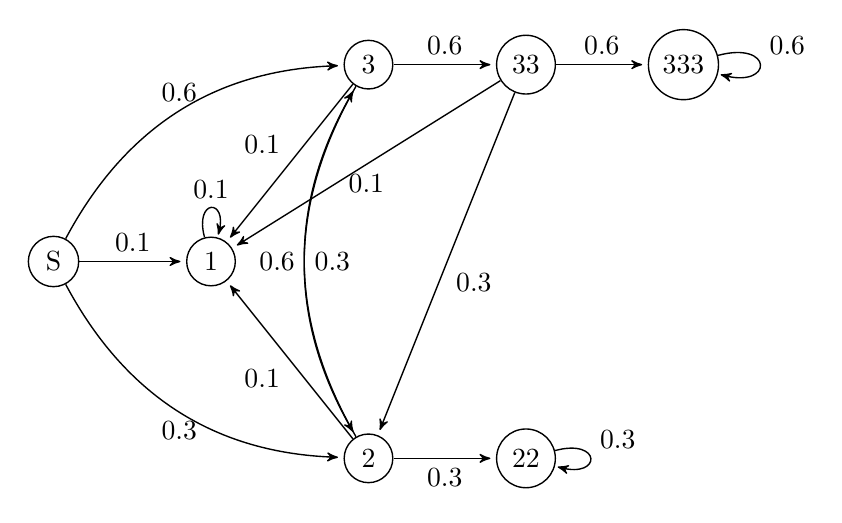
\begin{tikzpicture}[->, >=stealth', auto, semithick, shorten >=2pt, line width =0.5pt, node distance =2cm]
                        \node [circle , draw] (S) at (-4, 0) {S};
                        \node [circle , draw] (one) at (-2, 0) {1};
                        \node [circle , draw] (two) at (0, -2.5) {2};
                        \node [circle , draw] (ttwo) at (2, -2.5) {22};
                        \node [circle , draw] (three) at (0, 2.5) {3};
                        \node [circle , draw] (tthree) at (2, 2.5) {33};
                        \node [circle , draw] (ttthree) at (4, 2.5) {333};
                        \path (S) edge node [above] {$0.1$} (one);
                        \path (two) edge node [below left] {$0.1$} (one);
                        \path (two) edge node [below] {$0.3$} (ttwo);
                        \path (three) edge node [above left] {$0.1$} (one);
                        \path (three) edge node [above] {$0.6$} (tthree);
                        \path (tthree) edge node [below] {$0.1$} (one);
                        \path (tthree) edge node [below right] {$0.3$} (two);
                        \path (tthree) edge node [above] {$0.6$} (ttthree);

                        \path (S) edge [bend right] node [below] {$0.3$} (two);
                        \path (S) edge [bend left] node [above] {$0.6$} (three);

                        \path (two) edge [bend left] node [left] {$0.6$} (three);
                        \path (three) edge [bend right] node [right] {$0.3$} (two);
                        
                        \path (one) edge [loop above] node [above] {$0.1$} (one);
                        \path (ttwo) edge [loop right] node [above right] {$0.3$} (ttwo);
                        \path (ttthree) edge [loop right] node [above right] {$0.6$} (ttthree);
                    \end{tikzpicture}
                    \label{fig:markovchain_no3}
                \end{center}

                \end{solution}
                \begin{minipage}[t]{.9\textwidth}
                    \begin{lstlisting}[title=Code]
no3.P <- matrix(c(0, 0.1, 0.3, 0, 0.6, 0, 0,
                    0, 1, 0, 0, 0, 0, 0,
                    0, 0.1, 0, 0.3, 0.6, 0, 0,
                    0, 0, 0, 1, 0, 0, 0,
                    0, 0.1, 0.3, 0, 0, 0.6, 0,
                    0, 0.1, 0.3, 0, 0, 0, 0.6,
                    0, 0, 0, 0, 0, 0, 1),
                  nrow = 7, ncol = 7, byrow = TRUE)
no3_names <- c("S", "1", "2", "22", "3", "33", "333")

plotmat(t(no3.P),
        name = c(0, 1, 2, 3, 4, 5, 6, 7), shadow.size = 0, curve = 0.05,
        arr.length=0.5, arr.width=0.2, box.col="cornsilk", box.lwd=1, 
        box.prop=0.5, box.size=0.035, box.type="rect", box.cex=1, 
        cex.txt=0.7, lwd=0.5, self.cex=0.6)
                    \end{lstlisting}
                \end{minipage}
                \newline
                \begin{minipage}[t]{.9\textwidth}
                    \begin{lstlisting}[title=Output]

                    \end{lstlisting}
                \end{minipage}
            \part Calculate the probabilities $pa$, $pb$, and $pc$ of the sequences $a$, $b$ or $c$ first appearing
                \begin{solution}
                \\Hitting probabilities dari state S ke 333, state S ke 22 dan state S ke 1 dimana $h_{S,1} = 1 - h_{S,333} - h_{S,22}$. Model $h_{S,333}$ dengan $h_{333,333} = 1$ dan $h_{1,333} = h_{22,333} = 0$, 
                \begin{align*}
                    h_{S,333} &= 0.1h_{1,333} + 0.3h_{2,333} + 0.6h_{3,333} \\ h_{2,333} &= 0.1h_{1,333} + 0.3h_{22,333} + 0.6h_{3,333} \\ h_{3,333} &= 0.1h_{1,333} + 0.3h_{2,333} + 0.6h_{33,333}  \\ h_{33,333} &= 0.1h_{1,333} + 0.3h_{2,333} + 0.6h_{333,333} 
                \end{align*}
                Model $h_{S,22}$ dengan $h_{22,22} = 1$ dan $h_{1,22} = h_{333,22} = 0$,
                \begin{align*}
                    h_{S,22} &= 0.1h_{1,22} + 0.3h_{2,22} + 0.6h_{3,22}\\ h_{2,22} &= 0.1h_{1,22} + 0.3h_{22,22} + 0.6h_{3,22} \\ h_{3,22} &= 0.1h_{1,22} + 0.3h_{2,22} + 0.6h_{33,22}  \\ h_{33,22} &= 0.1h_{1,22} + 0.3h_{2,22} + 0.6h_{333,22} 
                \end{align*}
                Penyelesaian, $h_{S,333} = 0.3944, h_{S,22} = 0.2478$ lalu $h_{S,1} = 1 - h_{S,333} - h_{S,22} = 1 - 0.3944 - 0.2478 = 0.3578$
                \\Maka, probabilitas lottery wheel mendapat a sebesar 0.3578 dan mendapatkan b sebesar 0.2478, sedangkan c sebesar 0.3944
                \end{solution}
                \begin{minipage}[t]{.9\textwidth}
                    \begin{lstlisting}[title=Code]
no3.mcs <- new("markovchain", transitionMatrix = no3.P, states = no3_names)
no3.hit_prob = round(hittingProbabilities(no3.mcs), 4)
round(no3.hit_prob[1,], 4)
                    \end{lstlisting}
                \end{minipage}
                \newline
                \begin{minipage}[t]{.9\textwidth}
                    \begin{lstlisting}[title=Output]
     S      1      2     22      3     33    333 
0.0000 0.3579 0.5880 0.2478 0.7800 0.5707 0.3944 
                    \end{lstlisting}
                \end{minipage}
            \part Calculate the mean waiting time for the sequence $c$ to appear.
                \begin{solution}
                [Mungkin ini maksud soal 'Mean Absorption Time', karena 'Mean Waiting Tim' membutuhkan parameter $\lambda$ dan $\mu$]
                \begin{align*}
                    m_{iA} &= E[N_A|X_0 = i] \\ &= 
                    \begin{cases} 1 + \sum_{j\in S} P_{ij}m_{jA} & \text{if } i\notin A \\ 0 & \text{if } i \in A
                    \end{cases}
                \end{align*}
                Diketahui A = {1, 22, 333} sebagai set dari Absorbing State, dengan $m_{1A} = m_{22,A} = m_{333,A} = 0$, model menjadi
                \begin{align*}
                    m_{S,A} &= 1 + 0.1m_{1,A} + 0.3m_{2,A} + 0.6m_{3,A} \\ m_{2,A} &= 1 + 0.1m_{1,A} + 0.3m_{22,A} + 0.6m_{3,A} \\ m_{3,A} &= 1 + 0.1m_{1,A} + 0.3m_{2,A} + 0.6m_{33,A} \\ m_{33,A} &= 1 + 0.1m_{1,A} + 0.3m_{2,A} + 0.6m_{333,A}
                \end{align*}
                Penyelesaian, $m_{S,A} = 3.578652, m_{2,A} = 2.752809, m_{3,A} = 2.921348$ dan $m_{33,A} = 1.825843$
                \\Maka, mean absorbing time lottery wheel dari state S selama 3.578652, dari state 2 selama 2.752809, dari state 3 selama 2.921348 dan dari state 33 selama 1.825843
                \end{solution}
                \begin{minipage}[t]{.9\textwidth}
                    \begin{lstlisting}[title=Code]
meanAbsorptionTime(no3.mcs)
                    \end{lstlisting}
                \end{minipage}
                \newline
                \begin{minipage}[t]{.9\textwidth}
                    \begin{lstlisting}[title=Output]
       S        2        3       33 
3.578652 2.752809 2.921348 1.825843
                    \end{lstlisting}
                \end{minipage}
        \end{parts}
        
    \question Consider a linear birth-death process with birth rate 2.7 and death rate 0.6. We assume that the process starts in state 1.
        \begin{parts}
            \part Describe the state-space of the birth-death process. 
                \begin{solution}
                \\Poisson process merupakan contoh continuous-time Markov chain yang memiliki state 0, 1, 2, ... akan selalu berproses dari state n ke n+1, dimana $n \geq 0$. Proses seperti ini dikenal sebagai \textit{pure birth process} karena ketika transisi terjadi, sistem dari state selalu bertambah satu. 
                \\Secara umum, model eksponensial yang dapat bergerak (dalam satu transisi) hanya dari state n ke state n-1 atau state n+1 disebut \textit{birth and death model}. Untuk model seperti itu, transisi dari state n ke n+1 ditetapkan sebagai kelahiran, dan transisi dari state n ke n-1 sebagai kematian.
                \end{solution}
                
            \part Compute the probability that the process will be in state 5 at time 3. 
                \begin{solution}
                \\Probabilitas suatu proses sekarang berasa di state n pada waktu t dinotasikan sebagai $P_n(t)$. Dengan initial condition $P_0(t)$,
                \begin{align*}
                    P_0(t) &= \frac{\mu e^{(\lambda - \mu)t} - \mu}{\lambda e^{(\lambda - \mu)t} - \mu} \\ P_0(t = 3) &= \frac{0.6 e^{(2.7 - 0.6)3} - 0.6}{2.7 e^{(2.7 - 0.6)3} - 0.6} \\ &= 0.2219
                \end{align*}
                \begin{align*}
                    P_n(t) &= (1 - P_0)(1 - \frac{\lambda}{\mu}P_0) \Bigr(\frac{\lambda}{\mu}P_0 \Bigr)^{n-1} \\ P_5(t = 3) &= (1 - 0.2219)(1 - \frac{2.7}{0.6}0.2219) \Bigr(\frac{2.7}{0.6}0.2219 \Bigr)^{5-1} \\ &= 0.0011
                \end{align*}
                Maka, probabilitas birth-death process akan memasuki state 5 pada waktu 3 adalah 0.0011
                \end{solution}
                \begin{minipage}[t]{.9\textwidth}
                    \begin{lstlisting}[title=Code]
lambda = 2.7
mu = 0.6
state = 5
time = 3

no4.P0 = (mu*exp((lambda - mu)*time) - mu)/(lambda*exp((lambda - mu)*time) - mu)
round(no4.P0, 4)
Sol4.b = (1 - no4.P0)*(1 - no4.P0*(lambda)/(mu))*(no4.P0*(lambda)/(mu))^(state-1)
round(Sol4.b, 4)
                    \end{lstlisting}
                \end{minipage}
                \newline
                \begin{minipage}[t]{.9\textwidth}
                    \begin{lstlisting}[title=Output]
[1] 0.2219
[1] 0.0011
                    \end{lstlisting}
                \end{minipage}

            \part Find the mean and variance of the process at time 3.
                \begin{solution}
                \begin{align*}
                    E[X(t)] &= e^{(\lambda - \mu)t} \\ &= e^{(2.7 - 0.6)3} \\ &= 544.5719
                \end{align*}
                \begin{align*}
                    Var[X(t)] &= \frac{\lambda + \mu}{\lambda - \mu}e^{(\lambda - \mu)t}(e^{(\lambda - \mu)t} - 1) \\ &= \frac{2.7 + 0.6}{2.7 - 0.6}e^{(2.7 - 0.6)3}(e^{(2.7 - 0.6)3} - 1) \\ &= 465164.8
                \end{align*}
                \\Maka, nilai mean dari birth-death process adalah 544.5719, sedangkan nilai variansi dari birth-death process adalah 465164.8
                \end{solution}
                \begin{minipage}[t]{.9\textwidth}
                    \begin{lstlisting}[title=Code]
no4.mean = exp((lambda - mu)*time)
no4.var = (lambda + mu)/(lambda - mu)*exp((lambda - mu)*time)*(exp((lambda - mu)*time) - 1)
no4.mean
no4.var
                    \end{lstlisting}
                \end{minipage}
                \newline
                \begin{minipage}[t]{.9\textwidth}
                    \begin{lstlisting}[title=Output]
[1] 544.5719
[1] 465164.8
                    \end{lstlisting}
                \end{minipage}
        \end{parts}
        
    \question Consider that an acitivity of college student can be modeled as a four statemarkov chain: attending class, studying, socializing with friend, and participating in extracurricular activities. At one time, he attends class for average 2 hours then he either studying or socializing with friend with equal probability. He studies for average 30 minutes then with chance 40:30:30, he will attend class, hang-out with friend, or
        do the other activities. In average, he is socializing with friend for about an hour. After that, he will attend class (50\%), study (20\%), or participate in extracurricular activities (30\%). After participate in extracurricular activities for average 1.5 hours, he will attend class or study with a chance 80:20.
        \begin{parts}
            \part Calculate the limiting probabilities.
                \begin{solution}
                $$\mathbf{P}=\left(\begin{array}{cccc}0 & 0.5 & 0.5 & 0 \\ 0.4 & 0 & 0.3 & 0.3 \\ 0.5 & 0.2 & 0 & 0.3 \\ 0.8 & 0.2 & 0 & 0 \end{array}\right)$$
                Sebelumnya, definisikan state sebagai 0 \{masuk kelas\}, 1 \{belajar\}, 2\{bersosialisasi\} dan 3\{ekstrakurikuler\}. Proses Continuous-time Markov Chain akan menghabiskan waktu di tiap state dengan rate $v$. Apabila dinyatakan dalam satuan jam, didapatkan $v_0 = \frac{60}{120} = \frac{1}{2}$, $v_1 = \frac{60}{30} = 2$, $v_2 = \frac{60}{60} = 1$ dan $v_3 = \frac{60}{90} = \frac{2}{3}$
                $$v_i = \Bigr(\frac{1}{2} \quad2 \quad1 \quad\frac{2}{3}\Bigr)$$
                Diberikan persamaan General Transition Probabilities, $$q_{ij} = v_i P_{ij}$$ dan harus memenuhi $\sum_j P_{ij} = 1$, lalu $P_0 + P_1 + P_2 + P_3 = 1$.
                \begin{align*}
                    (\text{rate Proses Keluar})_0 &= (\text{rate Proses Masuk})_0 \\ q_{ij} &= v_i P_{ij} \\ \frac{1}{2}P_0 &= \left(\begin{array}{cccc}0 & 2 & 1 & \frac{2}{3} \end{array}\right) \cdot \left(\begin{array}{c}0 \\ 0.4P_1 \\ 0.5P_2 \\ 0.8P_3 \end{array}\right) \\ \frac{1}{2}P_0 &= \frac{4}{5}P_1 + \frac{1}{2}P_2 + \frac{8}{15}P_3
                \end{align*}
                Berlaku juga untuk state 1, 2 dan 3. Sehingga akan didapatkan Balance Equations
                \begin{align*}
                    \text{state}& \quad& \text{rate Proses Keluar} &= \text{rate Proses Masuk} \\ & 0 & \frac{1}{2}P_0 &= \frac{4}{5}P_1 + \frac{1}{2}P_2 + \frac{8}{15}P_3 \\ & 1 & 2P_1 &= \frac{1}{4}P_0 + \frac{1}{5}P_2 + \frac{2}{15}P_3 \\ & 2 & P_2 &= \frac{1}{4}P_0 + \frac{3}{5}P_1 \\ & 3 & \frac{2}{3}P_3 &= \frac{3}{5}P_1 + \frac{3}{10}P_2
                \end{align*}
                Tulis ulang melalui persamaan Transition Probabilities, $r_{ij} = \begin{cases} q_{ij} & \text{if } i\neq j \\ -v_i & \text{if } i = j \end{cases}$
                $$\mathbf{R} = \left(\begin{array}{cccc}-\frac{1}{2} & \frac{1}{4} & \frac{1}{4} & 0 \\ \frac{4}{5} & -2 & \frac{3}{5} & \frac{3}{5} \\ \frac{1}{2} & \frac{1}{5} & -1 & \frac{3}{10} \\ \frac{8}{15} & \frac{2}{15} & 0 & -\frac{2}{3} \end{array}\right)$$
                Penyelesaian menggunakan metode aproksimasi 
                $$\mathbf{P} = e^{\mathbf{R}t} = \biggr[\Bigr(\mathbf{I} - \mathbf{R}\frac{t}{n}\Bigr)^{-1}\biggr]^n$$
                dengan $P_0 = 0.5352$, $P_1 = 0.0978$, $P_2 = 0.1925$ dan $P_3 = 0.1746$
                \end{solution}
                \begin{minipage}[t]{.9\textwidth}
                    \begin{lstlisting}[title=Code]
no5.P <- matrix(c(-0.5, 0.25, 0.25, 0,
                  0.8, -2, 0.6, 0.6,
                  0.5, 0.2, -1, 0.3,
                  8/15, 2/15, 0, -2/3),
                nrow = 4, ncol = 4, byrow = TRUE)
round(expm(25*no5.P), 4) #Ambil angka t berapapun selama bisa mencapai limiting probabilities
                    \end{lstlisting}
                \end{minipage}
                \newline
                \begin{minipage}[t]{.9\textwidth}
                    \begin{lstlisting}[title=Output]
       [,1]   [,2]   [,3]   [,4]
[1,] 0.5352 0.0978 0.1925 0.1746
[2,] 0.5352 0.0978 0.1925 0.1746
[3,] 0.5352 0.0978 0.1925 0.1746
[4,] 0.5352 0.0978 0.1925 0.1746
                    \end{lstlisting}
                \end{minipage}

            \part Given that he is currently attending class, calculate the probability that he will pariticipate in extracurricular activities after 3 hours.
                \begin{solution}
                \begin{align*}
                    e^{\mathbf{R}(t=3)} &= \mathbf{P}(t=3) \\ &= \left(\begin{array}{cccc}0.5564 & 0.0999 & 0.1995 & 0.1443 \\ 0.5195 & 0.0976 & 0.1893 & 0.1936 \\ 0.5068 & 0.0960 & 0.2079 & 0.1893 \\ 0.5101 & 0.0934 & 0.1558 & 0.2408 \end{array}\right) 
                \end{align*}
                Kemudian, $\mathbf{P}_{03}(t=3) = 0.1443$
                \\Maka, probabilitas siswa akan mengikuti ekstrakurikuler setelah memasuki kelas 3 jam kemudian adalah 0.1443 
                \end{solution}
                \begin{minipage}[t]{.9\textwidth}
                    \begin{lstlisting}[title=Code]
Sol5.b = expm(3*no5.P)
round(Sol5.b[1, 4], 4)
                    \end{lstlisting}
                \end{minipage}
                \newline
                \begin{minipage}[t]{.9\textwidth}
                    \begin{lstlisting}[title=Output]
[1] 0.1443
                    \end{lstlisting}
                \end{minipage}

            \part Is the markov chain time reversible?
                \begin{solution}
                \\Markov chain dikatakan reversible jika memenuhi $$\pi_i P_{ij} = \pi_j P_{ij}$$ untuk semua i, j dengan $\pi$ merupakan steady-state distribution dan memiliki total peluang 1. 
                \\Namun, matrik probabilitas transisi $\mathbf{P}$ tidak reversible karena tiap baris matriks tersebut berjumlah 0.
                \end{solution}
                \begin{minipage}[t]{.9\textwidth}
                    \begin{lstlisting}[title=Code]
revers_check <- function(mcs){
  if(any(is(mcs) != "markovchain")){
    stop("Object is not a markov chain.")
  }
  result <- TRUE
  n <- nrow(mcs)
  steady <- steadyStates(mcs)
  for(i in 1:(n-1)){
    for(j in (i+1):n){
      if(steady[i]*mcs[i,j] - steady[j]*mcs[j,i] > 10^(-10)){
        result <- FALSE
        break
      }
    }
  }
  return(result)
}

no5.mcs <- new("markovchain", transitionMatrix = no5.P, states = as.character(0:3))
revers_check(no5.mcs)
                    \end{lstlisting}
                \end{minipage}
                \newline
                \begin{minipage}[t]{.9\textwidth}
                \begin{lstlisting}[title=Output, rulecolor=\color{red}]
Error in validObject(.Object) :
 invalid class "markovchain" object: Error! Rows of transition matrix do not sum to one
                \end{lstlisting}
            \end{minipage}
        \end{parts}
\end{questions}

\end{document}
